% This is samplepaper.tex, a sample chapter demonstrating the
% LLNCS macro package for Springer Computer Science proceedings;
% Version 2.20 of 2017/10/04
%
\documentclass[runningheads]{llncs}
\usepackage{soul}
\usepackage{wrapfig}
\usepackage{graphicx}
\usepackage{booktabs} % For formal tables
\usepackage{minted}
\usepackage{multirow}
\usepackage{graphicx}
\usepackage{subcaption}
\usepackage{amssymb}
\usepackage{amsmath}
\usepackage{verbatim}
\usepackage{textcomp}
\captionsetup{compatibility=false}
\usepackage{hyperref}
% Used for displaying a sample figure. If possible, figure files should
% be included in EPS format.
%
% If you use the hyperref package, please uncomment the following line
% to display URLs in blue roman font according to Springer's eBook style:
% \renewcommand\UrlFont{\color{blue}\rmfamily}

\begin{document}
%
\title{ \textit{BTestBox} - A tool for testing B translators and coverage of B models}
%
%\titlerunning{Abbreviated paper title}
% If the paper title is too long for the running head, you can set
% an abbreviated paper title here
%
\author{Diego de Azevedo Oliveira \inst{1} \and %\orcidID{0000-1111-2222-3333} \and
Val{\'e}rio Medeiros Jr\inst{2}\orcidID{0000-0001-6255-5026} \and
David D{\'e}harbe\inst{3}\and %\orcidID{2222--3333-4444-5555} \and
Martin A. Musicante \inst{1}\orcidID{0000-0001-5589-3895}
}
%
\authorrunning{D. Azevedo et al.}
% First names are abbreviated in the running head.
% If there are more than two authors, 'et al.' is used.

% \institute{Universit{\'e} de Sherbrooke, Canada\\
% \email{diegodeazevedooliveira@gmail.com}
% \and
% Instituto Federal de Educa{\c c}{\~a}o, Ci{\^e}ncia e Tecnologia do Rio Grande do Norte, Brazil\\
% \email{valerio.medeiros@ifrn.edu.br} \and
% Clearsy System Engineering, France\\
% \email{david.deharbe@clearsy.com}
% \and
% Universidade Federal do Rio Grande do Norte, Brazil\\
% \email{mam@dimap.ufrn.br}}

\institute{Universidade Federal do Rio Grande do Norte, Brazil\\
\email{diegodeazevedooliveira@gmail.com}, \email{mam@dimap.ufrn.br}
\and
Instituto Federal de Educa{\c c}{\~a}o, Ci{\^e}ncia e Tecnologia do Rio Grande do Norte, Brazil\\
\email{valerio.medeiros@ifrn.edu.br} \and
Clearsy System Engineering, France\\
\email{david.deharbe@clearsy.com}}


%\institute{Université de Sherbrooke, Canada \and
%Springer Heidelberg, Tiergartenstr. 17, 69121 Heidelberg, Germany
%\email{lncs@springer.com}\\
%\url{http://www.springer.com/gp/computer-science/lncs} \and
%ABC Institute, Rupert-Karls-University Heidelberg, Heidelberg, Germany\\
%\email{\{abc,lncs\}@uni-heidelberg.de}}
%\end{comment}


%
\maketitle              % typeset the header of the contribution
%
\begin{abstract}
The argument of correctness in refinement-based formal software design often disregards source code analysis and code generation.
To mitigate the risk of errors in these phases,
certifications of regulation entities demand or recommend testing the
generated software using some code coverage criteria.
We propose improvements over  \textit{BTestBox}, a tool for automatic generation
of tests for software components developed with the B method.
 \textit{BTestBox} supports several code coverage criteria and code
generators for different languages.
The tool uses a constraint solver to produce tests, being able to
identify dead code and tautological branching conditions.
It also generates reports with different metrics and may be used as an
extension to the Atelier B (an IDE used to write
software for critical safety systems).
Our tool performs a double task: first, it acts on the B model, by
checking code coverage.
In a second moment, the tool performs the translation of lower level B
specifications into programming language code, runs tests and compares
their results with the expected output of the test cases.
The present version of  \textit{BTestBox} uses parallelisation techniques that
significantly improve its performance.
The results presented here are encouraging, showing performance
numbers that are one order of magnitude better than for the previous
version of the tool.

%\keywords{First keyword  \and Second keyword \and Another keyword.}
\keywords{Proofs, Model-based testing, Code coverage.}
\end{abstract}
%
%
%


\section{Introduction}

The B method of software development~\cite{abrial2005b} produces source code by the successive refinement from an abstract model. 
%Compatible compilers used to translate the code are not dependable, compilers' errors may silently introduce bugs from correct source code~\cite{leroy2009formal}.
Since compilers are, in general, not dependable, compiler errors may silently introduce bugs to correct source code~\cite{leroy2009formal}.
 \textit{BTestBox} tests the translated code and assures dependability of the translation. 
Additionally,  \textit{BTestBox} may help the verification process to find counterexamples.
Model-based testing (MBT) provides an approach for the automatic generation of test cases from models~\cite{dalal1999model}. 
Our tool uses MBT and seeks to satisfy several code coverage criteria.

%Using a formal method as B is one technique to guarantee the specification behaviour as the user wants.

Formal methods such as B have been used to assure the behaviour of a specification in many contexts over the years, mostly in the development of critical systems~\cite{leuschel:2005,valerio_thesis:2016}. 
B is based on the Dijkstra notes~\cite{dijkstra1976discipline}; it uses the generalised substitution theory~\cite{hoare2002proof} and an abstract machine notation. 
It supports a modular modelling:  every component has its own specified module with different levels of abstraction, starting with an abstract machine that is successively refined to a concrete implementation. 
The goal is to have a proven implementation. 
The B code needs to be translated into binary code.
This process can lead to errors and requires more attention. 

% \begin{comment} The B process is demonstrated in Figure \ref{fig:Bmethod}.

% \begin{figure*}
%     \centering
%     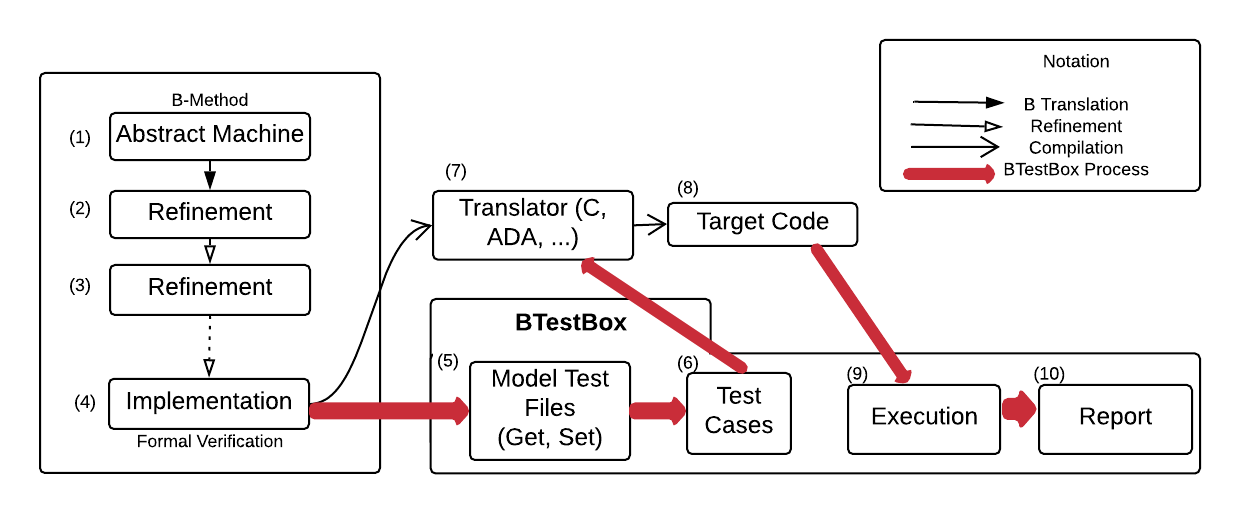
\includegraphics[width = \textwidth]{imagens/BMethodBTestBoxColor.png}
%     \caption{Overview of the B process with the  \textit{BTestBox} process.}
%     \label{fig:Bmethod}
% \end{figure*}
% \end{comment}

There exist translators to perform the conversion from B to a computer language such as C, ADA, and LLVM~\cite{deharbebtestbox}. 
Each of these translators takes a core subset of B as input language. 
%Moreover, a translator can have specific restrictions. %Such restrictions are not well documented and may confuse the user. 
%Additionally, compilers can insert bugs even with the correct source code~\cite{leroy2009formal}, and the code generators used with B demand additional safety criteria because they are employed in critical systems.

Testing techniques may supplement formal methods during the verification and validation process. 
They are used for an in-depth verification of the system. 
Software testing can quickly identify failures and expose defects introduced during code generation and code maintenance~\cite{deharbebtestbox}. 
Also, some certificates such as DO-178B, required by the Federal Aviation Administration (FAA), demand the use of software testing and measuring coverage over the code.

 \textit{BTestBox} may be used as an Atelier-B extension to automatically test B specifications. 
Our tool receives as input a B implementation, the target translator, one compiler, one coverage criterion, the folder project, and the logic expression solver (ProB ~\cite{1_leuschel_2017}) %\footnote{ProB is an animator, constraint solver and model checker for B models~\cite{1_leuschel_2017}.}
directory. 
Then,  \textit{BTestBox} generates test cases to cover the criterion.
The test cases are written in B, so that the models are translated and executed in any target language. 
Next, the results are compared with the expected values, producing a report. 
%In Figure \ref{fig:Bmethod} it is possible to observe where our tool fits in the B process.

In its current state,  \textit{BTestBox} is fully automatic and capable of testing translations from B implementations to C, checking for errors in the translation and reporting coverage rates for a number of criteria. 
%Each coverage has its functionality such as: identifying dead code with Code Coverage; logic tautology with functional coverages (Path and Branch coverage); and analysing the program flow with different logic decisions (Clause Coverage and MC/DC). 
%The tool and the results of an evaluation with the B language are presented in this paper. 
The two main contributions of  \textit{BTestBox} are: 
\textit{(i)} Supplying a full automatic model-based process for generation of executable criteria test cases for B implementations, thus avoiding the manual  construction of test cases; and
\textit{(ii)} Verifying the correctness of the B compiler while testing the translated code developed with the B formal method process using the supported criteria test cases consequently, it helps to find dead code and unnecessary conditions.

This article is organised as follows: 
Section \ref{sec:BTestBox} explains the  \textit{BTestBox} methodology, the background needed to understand the  \textit{BTestBox} process, how the tool works, and how it is associated with the B method. 
Section \ref{sec:Results} shows the results, metrics, threats, and limitations of our tool. 
Section \ref{sec:RelatedWork} describes the related work. 
Section \ref{sec:Conclusion} presents the conclusions and the future work.

\section{Methodology} \label{sec:BTestBox}

We present the applied methodology and the background needed to understand the process. 
Our tool tries to confirm the reliability of the B translator while executing the translated code with generated test cases to verify one coverage criterion.
\textit{BTestBox} takes one B implementation and tries to find test cases where one coverage criterion, chosen by the user, shall be achieved. 
To create the test cases, \textit{BTestBox} generates a control flow graph and uses Hoare's Logic to write a predicate which comprises the possible values for the execution paths, according to the chosen criterion. 
Then, the predicates are evaluated and the values of the input and output are stored for each valid solution. 
Our tool prepares components capable of executing and checking the execution of the test cases after the translation. Finally, the test components are translated and executed, and the metrics are reported.

\subsection{Path Generation}

This section describes how \textit{BTestBox} identifies the paths from a given B implementation. 
The process uses directed graphs and takes advantage of the B method properties. 
Edges of the graph are written as ($n_i$,$n_j$).
A path of a graph G is a sequence of nodes [$n_1$,$n_2$,\ldots,$n_M$], in which each adjacent pair of nodes ($n_i$, $n_{(i+1)}$), $1 \leq i < M$ is found in the $E$ set of edges.

Since B operations have one entry and one exit points, the control flow graphs have one start and one final node.
Different coverage criteria demand specific conditions to be attended by the control flow graph.
%Since the operations in B can only have one origin and has an end declaration. The initial and final set nodes of the graph for a given B operation are unitary test sets. 
% For some coverage criteria, it is required that the graph starts at one node and finishes at the other.
% This is only possible if the nodes are connected by a path. 
% When these coverage criteria are applied to specific graphs, they may produce paths that are impossible to execute. 
For each coverage criteria supported by \textit{BTestBox}, the tool can identify these conditions and possibly recognise dead code or useless guard clauses. 
\textit{BTestBox} supports the following criteria~\cite{ammann2008introduction}:
\textit{Statement Coverage} (ST); 
%: Criterion in which every command of the code shall be executed at least once~\cite{ammann2008introduction}. //
\textit{Branch Coverage} (BC);
%: To achieve this criterion, it is necessary to reach every branch in the control flow graph~\cite{ammann2008introduction}.//
\textit{Path Coverage} (PC);
%: It is necessary to reach all different paths in the control flow graph to achieve this coverage~\cite{ammann2008introduction}.//
\textit{Clause Coverage} (CC);
%: Given a predicate, each clause inside the predicate needs to be evaluated as either true or false at least once~\cite{ammann2003coverage}. //
\textit{Combinatorial Coverage} (CoC).
%: Given a predicate, each possible combination of the clauses shall be evaluated~\cite{ammann2003coverage}.

Generating a graph and the number of paths does not depend on which coverage criteria is chosen, but the number of paths needed to be executed depends on the coverage. 
Given the B implementation of the operation \texttt{RussMult} (Figure \ref{fig:russianMultImp}), \textit{BTestBox} draws the graph shown in Figure \ref{fig:russianMultGraph}.
% \begin{figure}[ht]
%         \centering
%         \begin{minipage}{0.58\textwidth}
%             \centering
        
%             \begin{minted}[escapeinside=||,mathescape=true,frame=single,firstnumber=1,linenos=false,breaklines,fontsize=\small]{ocaml}
% IMPLEMENTATION RussianMult_i
% REFINES RussianMult
% CONCRETE_VARIABLES  xx, yy, total
% INVARIANT  xx |$\in$| |$\mathbb{N}$| |$\wedge$| yy |$\in$| |$\mathbb{N}$| |$\wedge$| total |$\in$| |$\mathbb{N}$|
% INITIALISATION xx, yy, total := 0, 0, 0
% OPERATIONS
%   RussMult(aa,bb) = 
%     xx := aa; yy := bb; total := 0;
%     WHILE xx > 0 DO
%       IF xx mod 2 = 1 THEN total := total + yy END;
%       xx := xx / 2; yy := yy * 2
%     INVARIANT xx |$\in$| |$\mathbb{N}$| |$\wedge$| total + xx * yy = aa * bb
%     VARIANT xx
%     END
%   END
% END
%                 \end{minted}
%         \caption{Implementation of Russian multiplication.~\cite{schneider2001b}}
%         \label{fig:russianMultImp}
%     \end{minipage}%
% \end{figure}

% \begin{figure}[ht]
% \centering
% 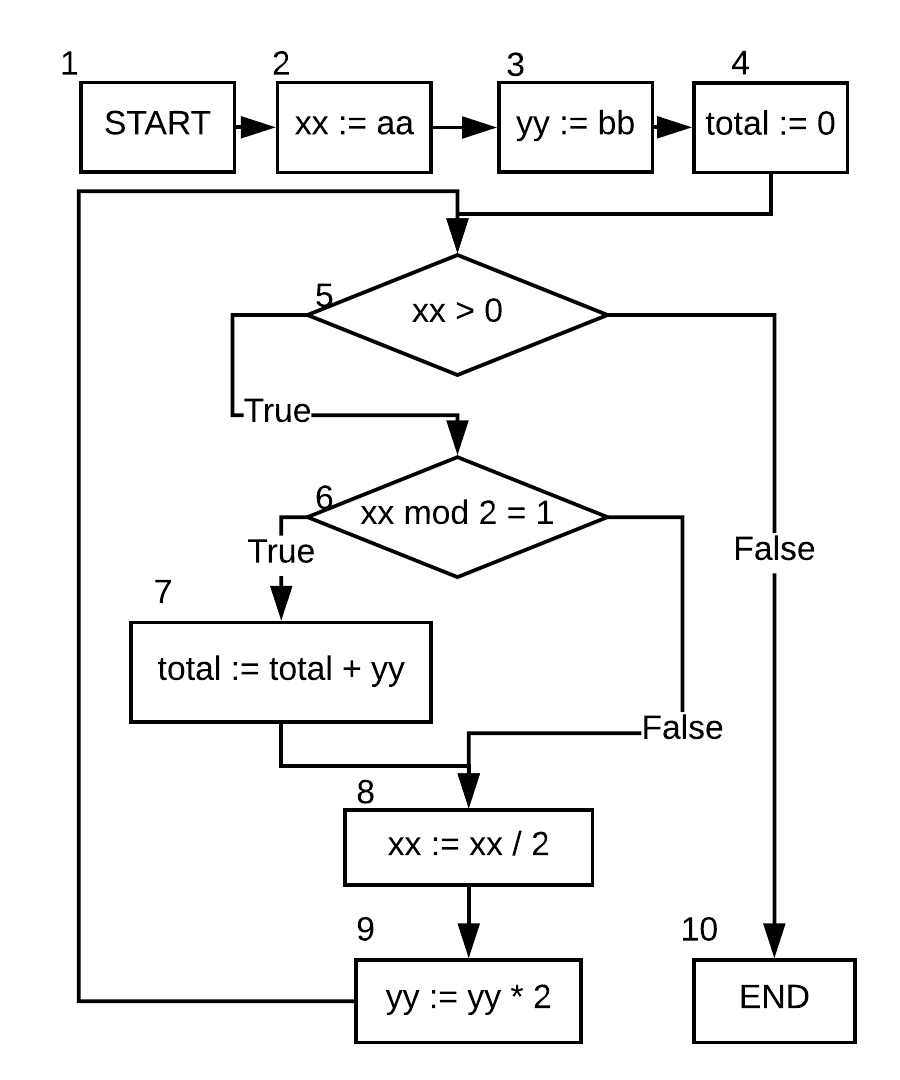
\includegraphics[width=0.45\textwidth]{imagens/lacoGrafo.png}
% \caption{Graph of the operation ``RussMult''.}
% \label{fig:russianMultGraph}
% \end{figure}
\begin{figure*}
\begin{minipage}{0.54\textwidth}
\begin{subfigure}{\textwidth}
\centering

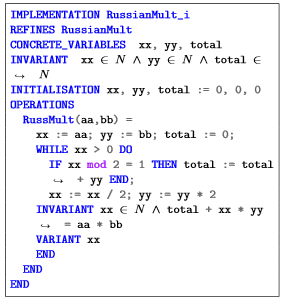
\includegraphics[width = \textwidth]{imagens/russianMult_i2.png}
\caption{Implementation.~\cite{schneider2001b}}
\label{fig:russianMultImp}
\end{subfigure}
\end{minipage}
\begin{minipage}{0.45\textwidth}
\begin{subfigure}{\textwidth}
\centering
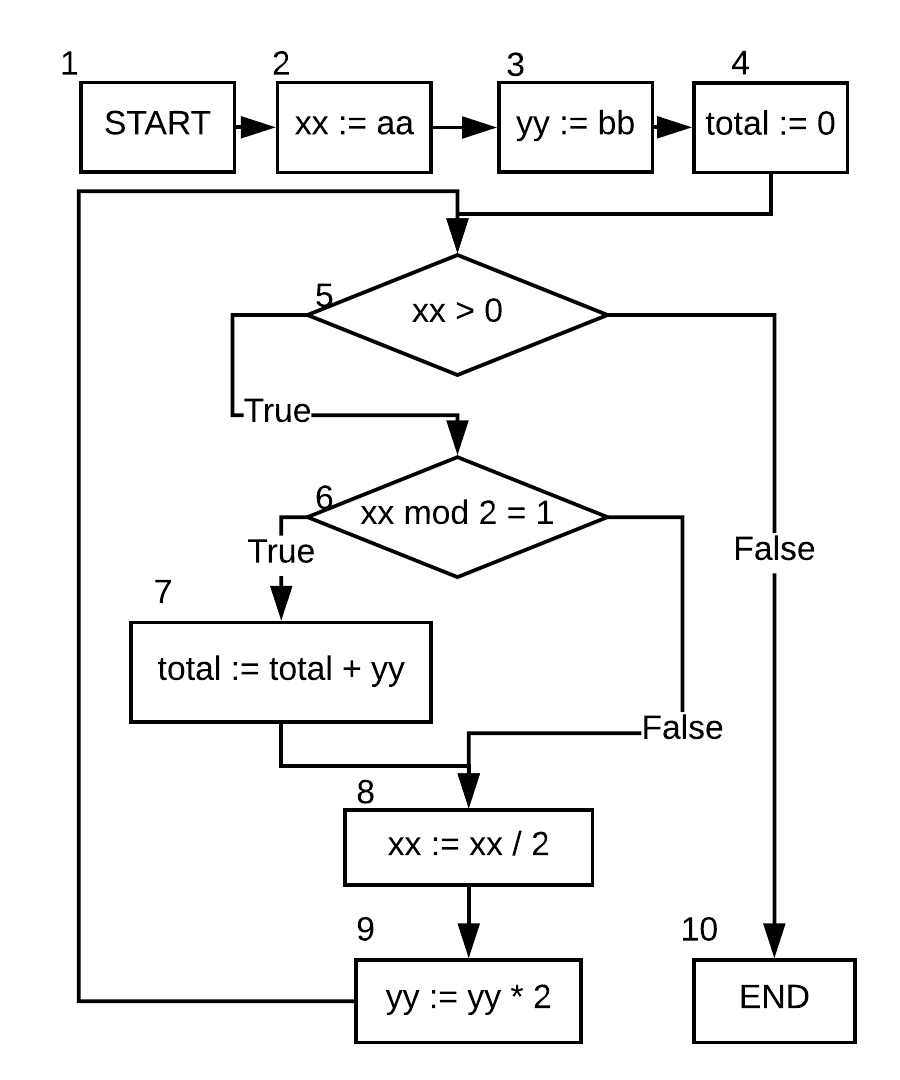
\includegraphics[width = \textwidth]{imagens/lacoGrafo.png}
\caption{Graph.}
\label{fig:russianMultGraph}
\end{subfigure}
\end{minipage}
\caption{Russia Multiplication Graph and Implementation.}
\end{figure*}
%Since the operation found in Figure \ref{fig:russianMultGraph} has a loop, it is possible to identify infinite paths and uncountable paths to test is not mechanically possible. 
Since the operation has a loop, it is possible to identify infinite paths. 
%However, testing uncountable paths is not mechanically possible.
To bypass this situation, our tool does not compute all the paths. Instead of repeating the instructions inside the loop and generating different paths for each time the loop is executed, \textit{BTestBox} counts the paths inside the loop once and uses them to represent all the paths created with the repetition of the loop. 
We assume this because of the B method property - a loop always has to end, and this is defined in the clauses of the B method. Then, we define that BTestbox generates the following paths: \textit{path 1} = \ul{1, 2, 3, 4, 5, 6, 7, 8, 9, 5, 10};  \textit{path 2} = \ul{1, 2, 3, 4, 5, 6, 8, 9, 5, 10} and \textit{path 3} = \ul{1, 2, 3, 4, 5, 10}.


\subsection{Writing Predicates} \label{writingPredicates}

During this section, we present how \textit{BTestBox} uses the Hoare\textquotesingle s logic to create a predicate. Our tool relays on the Hoare Triple, with which it is possible to calculate how a command can change the state. 
This form of the Triple is the notation: $\{P\} C \{Q\}$
% $$\{P\} C \{Q\} $$ 

\textit{P} represents the precondition for the execution of the command \textit{C}, and \textit{Q} is the post-condition established after the command. \textit{P} and \textit{Q} are states described in first-order logic. With those terms, it is possible to calculate the precondition by knowing the command and the post-condition. 

For writing the predicate, \textit{BTestBox} does a bottom-up approach with Hoare's Logic. We chose this approach because of the B method property for proved implementations, which implies that a proved implementation always has to finish. Since it is possible to assume that the operation is going to end, the post-condition \textit{Q} is assumable true at the last statement ``END'' of a B operation.

%In order to generate the test cases, \textit{BTestBox} writes the predicate related to each previous generated path of the model under test or until the chosen criteria is achieved. Even more, different criterion has separate goals, for example, with the PC is necessary to test every path and for the operation ``RussMult'' is necessary to test the three. Although, for ST if the path 1 is feasible, then just it need to be executed. Choosing the BC for the operation in the Figure \ref{fig:russianMultGraph}, the minimum necessary paths to be executed is two.

 \textit{BTestBox} writes the predicate to generate the test cases. They are related to each previously generated path of the model that are under test. They remain under testing until the chosen criterion is achieved. Further more, the different criterion has separate goals, for example, with the PC criterion: it is necessary to test every path, and for the ``RussMult'' operation, it is needed to test all the three paths. However, for the ST criterion, if path 1 is feasible, only then, it will be executed. By choosing the BC criterion for the operation in Figure \ref{fig:russianMultGraph}, the minimum necessary paths to be executed is two.

The \textit{BTestBox} procedure takes the path with the biggest amount of nodes to write the first predicate. Such consideration makes Path 1 the path under test. With the bottom-up approach, node 10 holds true and is the post-condition of the Hoare's Triple. Node 5 is the command. Since it needs to be a false guard, the value is the negative of the hold, generating the following scheme:
$\{P\} C \{Q\} \implies \{P\} [\neg(xx > 0)] \{true\} \implies P: xx <= 0 $

% $$\{P\} C \{Q\} \implies \{P\} [\neg(xx > 0)] \{true\} \implies P: xx <= 0 $$ 

After reaching node 5, since it is the guard of a loop, our tool divides the predicate into two: one partition for the inner part of the loop and the other for the outer part. The inner predicate is a post-condition indicating the values after running the loop and the outer is the previously calculated precondition for entering the loop. After calculating the inner predicate, both predicates are joined in a bigger predicate representing the post-condition of ending the operation. Then, \textit{BTestBox} first calculates the predicate for the inner part, and the post-condition refreshes to hold true because the loops in B have to reach an end. Differently from node 5, node 9 is not a guard, so it can change the previously established variables, but since it is a new predicate and holds it true, nothing will change:
$\{P\} C \{Q\} \implies \{P_i\} yy := yy * 2\{true\} \implies P_i: true$ 
% $$\{P\} C \{Q\} \implies \{P_i\} yy := yy * 2\{true\} \implies P_i: true $$

As it is possible to observe, the precondition remains the same as the post-condition. This happens because the variables in the statement do not manipulate the variables inside the post-condition and the command is not a guard. Such an effect occurs in the nodes 9, 8 and 7. Reaching the sixth node, the triple changes into the following:
$\{P\} C \{Q\} \implies \{P_i\} [xx\ mod\ 2=1]\{true\} \implies P_i: xx\ mod\ 2 = 1$ 
% $$ \{P\} C \{Q\} \implies \{P_i\} [xx\ mod\ 2=1]\{true\} \implies P_i: xx\ mod\ 2 = 1 $$ 

When arriving at the guard of the loop, our tool joins the external and the internal calculated predicates. Therefore, it also assumes a quantification over the values that are modified inside the loop. And due to the B declarations, it wraps the values of the variables in the quantification over the invariant. This assures that the assumed values satisfy the proved B implementation. Finally, the precondition is:
$P: \exists(xx, yy, total).(xx > 0 \wedge xx\ mod\ 2 = 1 \wedge xx \in \mathbb{N} \wedge total + xx * yy = aa * bb) \wedge \ \exists(xx, yy, total).((xx \leq 0) \wedge xx \in \mathbb{N} \wedge total + xx * yy = aa * bb)$ 
% $$ P: \exists(xx, yy, total).(xx > 0 \wedge xx\ mod\ 2 = 1 \wedge 
%  xx \in \mathbb{N} \wedge total + xx * yy = aa * bb)$$
% $$\wedge \  \exists(xx, yy, total).((xx \leq 0) \wedge xx \in \mathbb{N} \wedge total + xx * yy = aa * bb)$$

Then, \textit{BTestBox} continues to walk through the path, but the quantification cannot be changed by statements that appear after it. Since there are no more guards until node 1, the predicate will remain the same. With node 1, the invariant of the abstract machine ``RussianMult'' and the precondition of the abstract operation are added in the predicate: 
$P: \exists(xx, yy, total).(xx > 0 \wedge xx\ mod\ 2 = 1 \wedge xx \in \mathbb{N} \wedge total + xx * yy = aa * bb) \wedge \ \exists(xx, yy, total).(xx \leq 0 \wedge xx \in \mathbb{N} \wedge total + xx * yy = aa * bb) \wedge xx : NAT \wedge yy : NAT \wedge total : NAT \wedge aa : NAT \wedge bb : NAT$ 
% $$ P: \exists(xx, yy, total).(xx > 0 \wedge xx\ mod\ 2 = 1 \wedge
%  xx \in \mathbb{N} \wedge total + xx * yy = aa * bb)  $$
% $$ \wedge \ \exists(xx, yy, total).(xx \leq 0 \wedge xx \in \mathbb{N} \wedge total + xx * yy = aa * bb) \wedge$$
% $$ xx : NAT \wedge yy : NAT \wedge total : NAT \wedge aa : NAT \wedge bb : NAT$$

Subsequently, it is necessary to solve the found predicate to assure that it is a valid predicate and has at least one solution. Our tool is not able to solve predicate and retrieve the possible inputs of an operation and its respective output, so we used the \textit{ProB} constraint solver. The \textit{ProB} returned that a possible solution is aa = 1, bb = 0, xx = 0, yy = 0, total = 0. That way, the inputs of a test case is defined.

Getting the outputs is a similar process, but instead of the post-condition of the end node being true, its foo variables equals each input variable. Then:
$Q : foo\_aa = aa \wedge foo\_bb = bb \wedge foo\_xx = xx \wedge foo\_yy = yy \wedge foo\_total = total$ 
% $$Q : foo\_aa = aa \wedge foo\_bb = bb \wedge foo\_xx = xx \wedge
% foo\_yy = yy \wedge foo\_total = total$$

Writing a predicate and evaluating the outputs with the same process previously done returns the values foo\_aa = 1, foo\_bb = 0, foo\_xx = 0, foo\_yy = 0, foo\_total = 0. Finally, one test case is defined with the inputs and the expected outputs.

\textit{BTestBox} continues the process. It does the same for paths 1 and 2. Similarly, the predicate for the inputs of the second path is:
$P : \exists (xx, yy, total).(xx > 0 \wedge \neg(xx\ mod\ 2 = 1) \wedge xx \in \mathbb{N} \wedge total + xx * yy = aa * bb) \wedge \exists(xx, yy, total).(xx \leq 0 \wedge xx \in \mathbb{N} \wedge total + xx * yy = aa * bb) \wedge xx : NAT \wedge yy : NAT \wedge total : NAT \wedge aa : NAT \wedge bb : NAT$ 
% $$P: \exists(xx, yy, total).(xx > 0 \wedge \neg(xx\ mod\ 2 = 1) \wedge $$
% $$xx \in \mathbb{N} \wedge total + xx * yy = aa * bb) \wedge$$
% $$ \exists(xx, yy, total).(xx \leq 0 \wedge xx \in \mathbb{N} \wedge total + xx * yy = aa * bb) \wedge $$
% $$ xx : NAT \wedge yy : NAT \wedge total : NAT \wedge aa : NAT \wedge bb : NAT $$

The next step is to call \textit{ProB} and solve the predicate. The returned values for the inputs of the second path are aa = 2, bb = 0, xx = 0, yy = 0, total = 0. Identically, the outputs of path 2 are foo\_aa = 2, foo\_bb = 0, foo\_xx = 0, foo\_yy = 0, foo\_total = 0.

%After this procedure, \textit{BTestBox} found the necessary test cases for achieving BC for the operation ``RussMult''. And they are shown in the table \ref{tab:TestCases}.
After this procedure, \textit{BTestBox} found the necessary test cases for achieving the BC criterion for the ``RussMult'' operation, which are: \ul{aa = 1, bb = 0, xx = 0, yy = 0, total = 0 (Case test 1 - Input);  aa = 1, bb = 0, xx = 0, yy = 0, total = 0 (Case test 1 - Output)} and \ul{aa = 2, bb = 0, xx = 0, yy = 0, total = 0 (Case test 2 - Input);  aa = 2, bb = 0, xx = 0, yy = 0, total = 0 (Case test 2 - Output)}. 

%shown in Table \ref{tab:TestCases}.

\begin{comment}
\begin{table}
\centering
\caption{Test cases for ``RussMult''}
\begin{tabular}{c|c|c|c|c|}
\cline{2-5}
                                & \multicolumn{2}{c|}{Test 1} & \multicolumn{2}{c|}{Test 2} \\ \hline
\multicolumn{1}{|c|}{Variables} & Input        & Output       & Input        & Output       \\ \hline
\multicolumn{1}{|c|}{aa}        & 1            & 1            & 2            & 2            \\ \hline
\multicolumn{1}{|c|}{bb}        & 0            & 0            & 0            & 0            \\ \hline
\multicolumn{1}{|c|}{xx}        & 0            & 0            & 0            & 0            \\ \hline
\multicolumn{1}{|c|}{yy}        & 0            & 0            & 0            & 0            \\ \hline
\multicolumn{1}{|c|}{total}     & 0            & 0            & 0            & 0            \\ \hline
\end{tabular}
\label{tab:TestCases}
\end{table}
\end{comment}

\paragraph{Creating Test Case Files:} Our tool is capable of generating the test cases, inserting operations to manipulate the variables of an implementation under test, executing the translation, compare the results and report to the user. For this, \textit{BTestBox} creates copies of the user files and adds ``get'' and ``set'' operations. Also, it writes B components using the results of the evaluation of the predicates as the testing case files.

The evaluation occurs after the translation using a B compiler, with a compiler provided by the user and supported by our tool, \textit{BTestBox} can compile and execute the translated code. Finally, a HTML report file is generated and presented to the user, displaying the coverage metrics, showing which coverage objectives are not reached and a shortcut for all the files used on the test.

\begin{comment}

\subsection{Creating Test Case Files}


\marginpar{Talvez os 3 primeiros parágrafos possam ser modificados, acho que principalmente o segundo paragrafo}In this section, we describe how \textit{BTestBox} can manipulate the user files, insert ```get'' and ``set'' operations, and execute the test with the previously calculated inputs. 

Our tool copies the user files to keep the original B components and adds operations capable of changing the state of the variables. The ``set'' operation is responsible for setting the input values of variables that are defined and not used in the operation call. For the Russian multiplication implementation, the variables are xx, yy, and total. The ``get'' operations are responsible of providing the current state of each variable on the component. Every variable has a different ``get'' operation. Writing them to the model under test allows the \textit{BTestBox} to check the state of the variables and it compares with the expected output that was previously calculated.

The test cases are defined based on the chosen coverage criteria. Different criterion will likely result in diverse test cases. \textit{BTestBox} writes the test files capable of setting the test to a state defined in the test case in B. In a future process step, when the B files are translated to a computer language, all the test files are also translated using the same translator. The set test case has an operation for each test case scenario found during Section \ref{writingPredicates}. Such form allows it to test each test case in a different spot and makes it possible for the user to check when a failure is detected. Those operations call the operation under test with the inputs and create a auxiliary variable for storing and checking the values after the call. If the values are the same as expected, then the verdict ``true'' is returned, otherwise, the verdict is ``false''. Figure \ref{fig:SetTestModel} shows how the concrete set test operations are constructed. \marginpar{As figuras são bastante grandes, alguma solução para diminuí-las?}

% \begin{figure}
%     \centering
%     \begin{minipage}{0.46\textwidth}
%         \centering
        
%         \begin{minted}[frame=single,firstnumber=1,linenos=false,breaklines,fontsize=\small]{ocaml}
% OPERATIONS
%  verdict <-- TEST_1_RussMult =
%  BEGIN 
%   SetVarForTestRussMult(0,0,0);
%   VAR a1, a2, a3, a4, a5 IN
%   RussMult(1,0);
%   a1 <-- Get_xx; a2 <-- Get_yy;
%   a3 <-- Get_total;
%   a4 <-- Get_aa; a5 <-- Get_bb;
%   IF a1=0 AND a2=0 AND a3=0 AND
%       a4=1 AND a5=0 THEN
%     verdict := TRUE
%   ELSE verdict := FALSE END
%   END 
%  END;
%  verdict <-- TEST_2_RussMult =
%  BEGIN 
%   SetVarForTestRussMult(0,0,0);
%   VAR a1, a2, a3, a4, a5 IN
%   RussMult(2,0);
%   a1 <-- Get_xx; a2 <-- Get_yy;
%   a3 <-- Get_total;
%   a4 <-- Get_aa; a5 <-- Get_bb;
%   IF a1=0 AND a2=0 AND a3=0 AND
%       a4=2 AND a5=0 THEN
%     verdict := TRUE
%   ELSE verdict := FALSE END
%   END 
%                 \end{minted}
%         \caption{Concrete set test operations.}
%         \label{fig:SetTestModel}
%     \end{minipage}%
% \end{figure}

\begin{figure*}[ht]
\begin{minipage}{0.5\textwidth}
\begin{subfigure}{\textwidth}
\centering
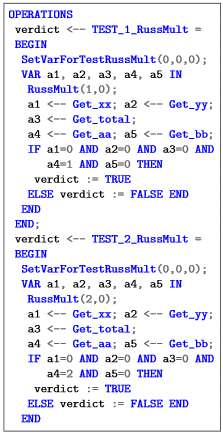
\includegraphics[width = \textwidth]{imagens/concreteSetTest.png}
\caption{Concrete set test operations.}
\label{fig:SetTestModel}
\end{subfigure}
\end{minipage}
\begin{subfigure}{0.49\textwidth}
\centering
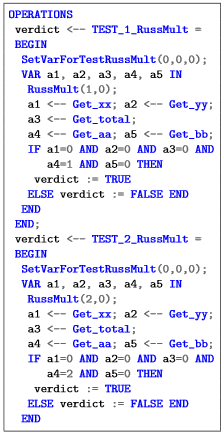
\includegraphics[width = \textwidth]{imagens/concreteRunTest.png}
\caption{Concrete run test operations.}
\label{fig:RunTestModel}
\end{subfigure}
\caption{Concrete test operations}
\end{figure*}

Once the B component for setting is written, our tool prepares another component capable of reading the answer of each test case operation. It can be found in Figure \ref{fig:RunTestModel}. The running of the test component implies in an approach to verify the B translator. Therefore, the user may have two possibilities of checking the compiler: the one automatically executed by \textit{BTestBox} or animating the B component responsible for running the test.

% \begin{figure}
%     \centering
%     \begin{minipage}{0.45\textwidth}
%         \centering
%         \begin{minted}[frame=single,firstnumber=1,linenos=false,breaklines,fontsize=\small]{ocaml}
% LOCAL_OPERATIONS
%   verdict <-- Test_RussMult =
%     ANY kk WHERE kk : BOOL THEN verdict := kk END;
% OPERATIONS
%   verdict <-- Test_RussMult =
%   BEGIN
%     VAR a1, a2 IN
%       a1 <-- TEST_1_RussMult;
%       a2 <-- TEST_2_RussMult;
%       IF a1 = TRUE & a2 = TRUE THEN
%         verdict := TRUE
%       ELSE verdict := FALSE END
%     END
%   END;
%   verdict <-- Test_All =
%   BEGIN 
%     VAR v0 IN
%       v0 <-- Test_RussMult;
%       IF v0 = TRUE THEN
%         verdict := TRUE
%       ELSE verdict := FALSE END
%     END
%   END
%         \end{minted}
%         \caption{Concrete run test operations.}
%         \label{fig:RunTestModel}
%     \end{minipage}
% \end{figure}

\marginpar{Descrevendo o processo, e porquê é necessario criar um main, talvez essa explicação possa sair.}In the \textit{BTestBox} usual process, the next step is the translation of the code by a B compiler. While using a B translator, it is necessary to create a main file - \textit{BTestBox} has the ability to write this piece of code. Finally, the code is translated, but it is not available for execution. Our tool also asks for a compiler, defined by the user, to create an executable file of the test. With the program of the test, it is possible to show the results of the execution in a new window for the user.

But that is not all: \textit{BTestBox} also writes an HTML file that provides a summary of the test. It has three sections: The first page, Figure \ref{fig:report1}, shows the tested operations and the test results with the percentage of coverage; the second page, Figure \ref{fig:report2}, contains the inputs and expected outputs for every test, it also reports which objective was not successfully achieved; the third page, \ref{fig:report3}, presents the library with the links for all files used in the test: original files, test files, and translated files. 

\begin{figure*}[ht]
\begin{minipage}{0.45\textwidth}
\begin{subfigure}{\textwidth}
\centering
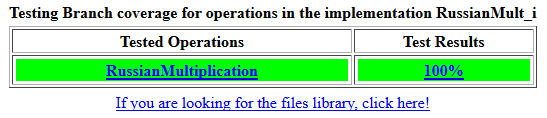
\includegraphics[natwidth=547,natheight=118,width = \textwidth]{imagens/reporte1.png}
\caption{First report page.}
\label{fig:report1}
\end{subfigure}
\begin{subfigure}{\textwidth}
\centering
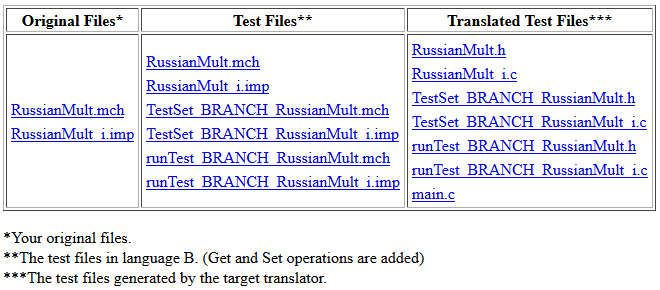
\includegraphics[natwidth=660,natheight=290,width = \textwidth]{imagens/reporte3.png}
\caption{Library report page.}
\label{fig:report3}
\end{subfigure}
\end{minipage}
\begin{subfigure}{0.50\textwidth}
\centering
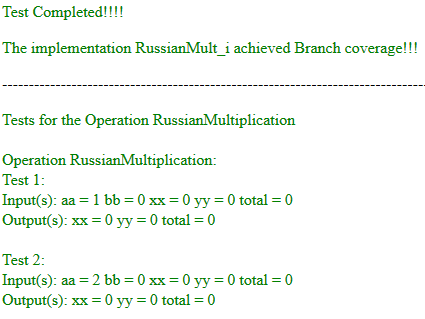
\includegraphics[natwidth=425,natheight=319,width = \textwidth]{imagens/reporte2.png}
\caption{Detailed report page.}
\label{fig:report2}
\end{subfigure}
\caption{Pages of the report}
\end{figure*}

\end{comment}

\section{Results} \label{sec:Results}

%This section is responsible for discussing the results, the validation, and the potential improvements.

\textit{BTestBox} was tested for a variety of different B clauses and structures, with the goal of assuring the correctness of the process and the functionality of the tool. Our tool ran more than 120 proved implementations. Additionally, one real B project granted by the \textit{ClearSy} enterprise was put under test. The groups of diverse components executed by our tool are presented below. The groups were divided regarding the language structure exercised with the B component.

\begin{comment}
\begin{table}[ht]
\centering
\caption{B Components Groups for validation.}
\begin{tabular}{l|c|}
\cline{2-2}
                                        & \multicolumn{1}{l|}{Quantity of implementations} \\ \hline
\multicolumn{1}{|l|}{Clauses}           & 14                                             \\ \hline
\multicolumn{1}{|l|}{Operation Call}    & 26                                             \\ \hline
\multicolumn{1}{|l|}{Depth one blocks} & 6                                              \\ \hline
\multicolumn{1}{|l|}{Depth two blocks} & 25                                             \\ \hline
\multicolumn{1}{|l|}{Depth three blocks} & 58                                             \\ \hline
\multicolumn{1}{|l|}{Industrial Confidential} & 1
\\ \hline
\end{tabular}
\label{tab:ValidationGroups}
\end{table}
\end{comment}


\begin{itemize}
    %\item The clause group exercises the structures sees, extends, constants, constraints, imports, promotes, sets, variables, and local operations. Those elements are put in test in groups and separately to observe the changes in the predicate that each can perform.
    \item The ``Clauses'' group with 14 examples exercises the \underline{sees}, \underline{extends}, \underline{constants}, \underline{constraints}, \underline{imports}, \underline{promotes}, \underline{sets}, \underline{variables} and \underline{operations}. Those elements are tested both in groups and separately. Those tests observe the changes that each element can perform in the predicate.
    %\item Operation calls employ the operation calls in different contexts.
    \item The ``Operation Call'' with 26 examples employs operation calls in different contexts.
    %\item Depth blocks are sensitive to the instructions if-else, case, skip, while and assignment. They are grouped and nested to max depth of three. 
    \item The ``Depth'' blocks with 89 examples are sensitive to the if-else, case, skip, while, and assignment instructions. They are grouped and nested to the maximum depth of three.
    %\item The industrial project is responsible for diverse contributions to \textit{BTestBox}, with B structures non previous tested. Unfortunately, the tests generated for this case are very time consuming due the necessity of sets expansions.
    \item The ``Industrial'' project with one big example is responsible for different contributions to the \textit{BTestBox}, with non-previously tested B structures. Unfortunately, the tests generated for this case are very time-consuming due to the necessity of set expansions.
\end{itemize}

All the presented implementation, excluding the industrial project, were exercised with all the coverage criteria supported by the \textit{BTestBox}. Even contributing to the development of our tool, the industrial project was not able to fully test the project because few data structures are not yet supported: matrices and trees. 
The current data structures and elements supported are: \textit{Arithmetic operators}; \textit{Logical operators};  \textit{Sets operators} and \textit{Vectors}.

\begin{comment}
\begin{table}
\centering
\caption{Structures supported by \textit{BTestBox}}
\label{tab:tabelaSuportados}
\begin{tabular}{|c|c|c|}
\hline
\multicolumn{2}{|c|}{Type}                     & Supports \\ \hline
\multicolumn{2}{|c|}{Arithmetic operators}   & $\surd$   \\ \hline
\multicolumn{2}{|c|}{Logical operators}       & $\surd$   \\ \hline
\multicolumn{2}{|c|}{Sets operators}  & $\surd$   \\ \hline
\multirow{3}{*}{Data structure} & Vectors  & $\surd$   \\ \cline{2-3} 
                                    & Matrices & X       \\ \cline{2-3} 
                                    & Trees  & X       \\ \hline
\end{tabular}
\end{table}
\end{comment}

Our tool was also tested with the intention of expliciting the problems of using the \textit{ProB} tool and the scalability of \textit{BTestBox}. To present that, giant B files were analysed and metrics were registered. A variety of lexical elements of the B language were created with nested instructions. They were designed to test the scalability of a B translator to LLVM~\cite{deharbebtestbox}. Those files may be classified by the number of nesting in command block of the operations. %the variable that define the generation of the files are the number of nesting in command block
The results are shown in Table \ref{tab:escalabilidade}.  
%and the quantity of blocks inside an operation. Such operations can be built around 1, 10, 50, 100 or 500 blocks and the nesting level varies between 1 and 5.

%For the scalability tests, was used a computer with the operating system Windows 10 64 bits, with a processor Intel Core i5\-6300HQ 2300 GHz and 8 GB de memória RAM. We observed that the scalability may stick to minor size implementations since the Atelier-B, version 4.3.1, available on the computer does not generate the proof obligations and the BXML tree file necessary for \textit{BTestBox}.
We initially used a computer with the Windows 10 64 bits operating system, with an Intel Core i56300HQ 2.300 GHz processor with 4 cores and 8 GB of RAM for the scalability tests. %We observed that the scalability might stick to a minor size implementations since the Atelier-B, version 4.3.1, available on the computer does not generate the proof obligations and the BXML tree files which are required for \textit{BTestBox}.
%
 %
To improve the results, we researched and implemented threads inside the tool.
This way, \textit{BTestBox} can execute its procedure to various operations at the same time.
This severally reduce the time for the predicate evaluation. In Table \ref{tab:escalabilidade}, it is possible to observe the results of tests using a computer with 2 CPUs Intel Xeon Sixteen-Core E5-2698v3 2.300 GHz allocating with a maximum 20 cores and 80 GB of RAM. The time process was reduced approximately by ten times.
All examples of Table \ref{tab:escalabilidade} can be easily executed in a leased cloud computer costing less than one US dollar with similar results.
Our experiments have shown that processing time is reduced approximately proportionally when we use a computer with more processing cores.

% \marginpar{Pode ser excluido?}Additionally, the implementation provided in~\cite{deharbebtestbox} had to be adapted to be properly used with \textit{BTestBox}, but it did not lose any nesting or instruction. Such adaptations are needed because the implementations are not proved. They present decisions that perform mathematical calculus without a solution. Also, they have operation calls. In the current state, our tool is not able to manage operation calls due to the necessity of using a close Atelier-B function that was only available during the process of validation.

%During the process of testing, it is notorious that the time for evaluation is longer than the other steps of \textit{BTestBox}. The results are shown in Table \ref{tab:escalabilidade}. It is possible to observe the amount of time spent for the evaluation with \textit{ProB}.

% \begin{table}[h!]
% \centering
% \caption{Implementations for scalability}
% \label{tab:escalabilidade}
% \begin{tabular}{|c|c|c|c|}
% \hline
% Component                                                                                          & COMP\_1seq1 & COMP\_2seq1 & COMP\_3seq1 \\ \hline
% \begin{tabular}[c]{@{}c@{}}Quantity of\\ operations\end{tabular}                                    & 39          & 199         & 999         \\ \hline
% %Nesting level                                                                                          & 1           & 2           & 3           \\ \hline
% %\begin{tabular}[c]{@{}c@{}}Commands\\ by block\end{tabular}                                         & 1           & 1           & 1           \\ \hline
% \begin{tabular}[c]{@{}c@{}}Execution time\\ with 4 cores\\ (seconds)\end{tabular}                       & 587      & 3102      & 18214     \\ \hline
% \begin{tabular}[c]{@{}c@{}}Execution time\\ with 20 cores\\ (seconds)\end{tabular}                       & 38     & 176     & 2286   \\ \hline
% \begin{tabular}[c]{@{}c@{}}Time reduced\\ for evaluation\end{tabular}            & 93\%     & 94\%     & 87\%     \\ \hline
% \end{tabular}
% \end{table}

\begin{table}[h!]
\centering
\caption{Implementations for scalability}
\label{tab:escalabilidade}
\begin{tabular}{|c|c|c|c|c|}
\hline
Component   & \begin{tabular}[c]{@{}c@{}}Quantity of \\ operations\end{tabular} & \begin{tabular}[c]{@{}c@{}}Execution time \\ with 4 cores\end{tabular} & \begin{tabular}[c]{@{}c@{}}Execution time \\ with 20 cores\end{tabular} & \begin{tabular}[c]{@{}c@{}}Reduced time\\ for evaluation\end{tabular} \\ \hline
COMP\_1seq1 & 39                                                                & 587 seconds                                                            & 38 seconds                                                              & 93\%                                                                  \\ \hline
COMP\_2seq1 & 199                                                               & 3102 seconds                                                           & 176 seconds                                                             & 94\%                                                                  \\ \hline
COMP\_3seq1 & 999                                                               & 18214 seconds                                                          & 2286 seconds                                                            & 87\%                                                                  \\ \hline
\end{tabular}
\end{table}

\begin{comment}


\section{Potential Improvements}


\marginpar{Recentes melhorias compatível com os sistemas operacionais Windows, Linux e OsX. Adição de threads e configuração para execução em servidor dedicado. }

In this Section we relate the possible points of improvements of the \textit{BTestBox}. All the mentioned improvements are planned and will be in the authors' future work.

In the current state, our tool supports five coverage criteria, and our study aims to add the Modified Condition/Decision Coverage (MC/DC). Since the Combinatorial Coverage is stronger than the MC/DC, our tool is already capable of generating tests that will achieve the MC/DC, but CoC is more time consuming since it demands more tests. It is possible to satisfy MC/DC without achieving CoC.

Currently, \textit{BTestBox} is only able to test the C compiler, the C4B with different translation profiles, and to use the compiler GCC, but it has plenty of space for development and with small improvements, it can include other B translators such as LLVM and ADA with the user of a correspondent compiler for executing the translated code. %The tool is also only available for Windows, but we plan to diffuse it for the Mac and Linux OS.

\marginpar{Candidato a cortar.} A problem happens when there is a machine that does not have an implementation. Usually, this is the case of base machines, and this limits the number of real projects which \textit{BTestBox} could be applied for. To accomplish that, \textit{BTestBox} has to deal with non-deterministic predicates. The procedure gets complicated when the tool is trying to test an implementation and wants to compare whether the output is the same as to when the \textit{ProB} evaluates the predicate. \textit{BTestBox} only accepts deterministic machines or implementations because we focus on deterministic tests. This is a conceptual limitation of any testing tool based on models.
\end{comment}
%\section{Threats to Validity}
% Esta seção muda de cenário quando temos novos experimentos e resultados. O que está escrito abaixo não contribui para aceitação do artigo e não é claro o suficiente sobre possíveis problemas gerando uma confusão ao leitor.

%Despite our efforts and the measures taken throughout our work to assure the functionality of our tool and the validity of our results, our study faces some threats to validity. Also, the validation of our tool faces limitations that may impact on the external validity.

%External validity alludes to the degree to which our experiments' results can be generalised. The most relevant and potential threat to the validity of \textit{BTestBox} is the population of the models tested with our tool. Since the models developed for testing \textit{BTestBox} are limited and made during the proper creation of our tool, it is not possible to assure the full correctness. Additionally, even concerning the number of tests, the tool needs maturation and to be operated by more users with different cases and situations.\marginpar{Desnecessário: ''the tool needs maturation and to be operated by more users with different cases and situations''}. Notwithstanding, related to the external validity, there is the necessity of employing a third party function that is not available in the regular distribution of the third party tool.

%%To address these potential threats, more studies will be expanded by the authors using a bigger range of models and a more powerful computer, reducing the time of tests and expanding the quantity number of models tested by \textit{BTestBox}.

\section{Related Work} \label{sec:RelatedWork}
%\marginpar{Um grande diferencial do \textit{BTestBox} em relação as outras ferramentas está na capacidade de gerar testes para cinco diferentes critérios de cobertura. Isso amplia as configurações de testes e pode ser melhor explorado no texto.}
Generating test cases from models is a subject that has been studied by research groups for several years. The work~\cite{shafique2010systematic} contains an interesting systematic review about testing a software system by using a test model of its behaviour, and it was useful to \textit{BTestBox}. Another important work is in~\cite{marinescu:2015}. Its authors showed a new overview of the current state of the art for model-based testing tools that use requirement-based specification languages. They quoted two tools compatible with the B method: ProTest~\cite{leuschel:2005} and BZ-TT~\cite{bouquet:2002}.

The \textit{BZ-TT} contains an environment for boundary-value test generation from Z and B specifications. This tool relies on constraint solving, and its goal is to test every operation of the system at every reachable boundary state. A boundary state is a system state in which at least one of the state variables has a maximum or minimum boundary value. It is not open source, and its last public news was in the year of 2003.

The \textit{ProB} is a tool with support to generate tests from B models. It has an automatic test environment for B specifications and a component called ProTest.
Its component uses model-checking techniques to find test sequences that satisfy its test generation parameters. The user has to define the requirements to be satisfied by the test cases. These requirements are operations that must be covered and predicates that must hold true at the end of each test case. The tool only generates abstract test cases that have to be implemented before they can be executed. \textit{BTestBox} is capable of generating executable test scripts. That is an advantage. 


The \textit{BETA}~\cite{ernesto_thesis:2016} generates test code using input space partitioning and logical coverage criteria. It also automates the generation tests and supports several coverage criteria. The generated tests are based on abstract B models, and some important information about the model are ignored.
Information ignored by \textit{BETA} may generate inaccurate tests related to the B concrete model. Differently, \textit{BTestBox} generates test cases directly from B concrete model which is a closer representation of the software.
Another relevant difference is that \textit{BETA} is focused on unit testing, while \textit{BTestBox} tests both approaches on unit testing and the entire module. Furthermore, \textit{BTestBox} has previous experiments with massive and random tests~\cite{deharbebtestbox}.

\section{Conclusions and Future Work} \label{sec:Conclusion}


Currently, \textit{BTestBox} is a free and open-source tool under Berkeley-licensed software.
This tool was born from an international collaboration between the academia and the software industry. The collaboration resulted in an initial version of the tool. Now, the goal is to increase the maturity of \textit{BTestBox} to deal with industrial applications.
The developed software is in continuous development and the tool offers an important contribution to the community.

Several components were created with different B structures to test the functionality and correctness of the \textit{BTestBox}. More than 120 B concrete models were created to test the B language, and one model, simulating a real used B program, was provided by \textit{ClearSy}. \textit{BTestBox} is already capable of generating tests that verify MC/DC. Our tool is capable of generating tests to verify the Combinatorial Coverage, since it demands the test of all possible combinations of guards, achieving CoC implies in being successful at MC/DC. %Unfortunately, CoC generates a high number of tests. Efforts are concentrated in developing an approach to generate fewer test cases and achieve the required coverage.

%BTestBox\textquotesingle s future research has to be towards improving the performance. This is a problem since it calls ProB and sometimes the model checker has to expand a big set or various sets. The time to run a predicate with many clauses is enormous in comparison with predicates without any expansion. To solve this, the predicate generated by \textit{BTestBox} has to be simplified with only the conditions that are bound to the variables that are used in operation.

%When considering the evaluation of the predicate, \textit{BTestBox} inherits every limitation from the logic expression solver (ProB). There are other candidate solvers that help to minimise the restrictions, and they will be studied.

Since  \textit{BTestBox} uses B translators, if the translator has any limitation to B language, it is also applied to our tool. However, there are several B translators, and the  \textit{BTestBox}'s approach is compatible with all of them, because the generated tests are also represented in B. 

Significant improvements were developed in the tool offering excellent results.
The parallelization techniques applied reduced the process time and extended the power to generate tests for larger samples. We also adjusted small configurations on the tool to run on a remote computer with more processor cores. Those improvement required changes that made our tool compatible with the most common operating systems (Microsoft’s Windows, Apple\textquotesingle s OS X and Linux distributions). All recent advances presented here are encouraging, showing performance numbers that are one order of magnitude better than for the previous version of the tool.

%The authors would like to thank ClearSy, IFRN, UFRN, CAPES and the anonymous referees for the support.

%\section*{Acknowledgement}
%  The authors would like to especially thank ClearSy System Engineering for providing the industrial case and support. The authors would also like to thank the anonymous referees for their valuable comments and helpful suggestions. The work is supported by the Federal Institute of the Rio Grande do Norte, the Federal University of Rio Grande do Norte and CAPES (Coordination of Improvement of Higher Level Personnel).
  %This work was grammatically reviewed by Antonio Henrique Nepomuceno Coelho (Federal English Teacher at IFRN).



%
% ---- Bibliography ----
%
% BibTeX users should specify bibliography style 'splncs04'.
% References will then be sorted and formatted in the correct style.
%

\bibliographystyle{splncs04}


\bibliography{bibs} 

\end{document}
